\documentclass{sosg-informe}

\graphicspath{{figuras/}{../../clima/pronostico/fase0/}}

\title{Pronóstico experimental de lluvia fuerte en Galápagos:\\evaluación y calibración de modelos globales (fase 0)}
\titulocorto{Pronóstico experimental de lluvia fuerte (fase 0)}
\numero{2026-08}
\estado{Borrador para discusión}
\titulocita{Pronóstico experimental de lluvia fuerte en Galápagos: evaluación y calibración de modelos globales (fase 0)}
\relacionados{Issues \issue{20}, \issue{30}, \issue{31}, \issue{46} y \issue{56} · repositorio mayait/sosgalapagos-datos}
\date{4 de noviembre de 2026}

\begin{document}
\maketitle

\begin{abstract}
Antes de publicar un pronóstico de lluvia en la plataforma de clima de SOS Galápagos se evaluó si los modelos meteorológicos globales sirven para anticipar los días de lluvia fuerte en las islas. Se comparó el archivo de corridas anteriores de siete modelos (ECMWF IFS y AIFS, GFS, ICON, UKMO, ARPEGE y GEM), de enero de 2024 a noviembre de 2026, con la lluvia diaria medida por el GSC-USFQ en la parte alta de San Cristóbal, por la FCD en Puerto Ayora y por la red IERSE-WSN en la parte alta de Santa Cruz. En milímetros los modelos se quedan muy cortos: la víspera del 30-oct-2026 daban 0--33~mm en la parte alta de Santa Cruz, donde llovieron 238~mm. Pero sí \enquote{suben} los días en que llueve fuerte. El \emph{consenso}, que promedia el percentil de cada modelo dentro de su propia climatología, distingue los días con 20~mm o más con un AUC de 0,85--0,92 en temporada lluviosa hasta pasado mañana, frente a 0,64 de la climatología y 0,54--0,74 de la persistencia. Una regresión logística por grupo, temporada y anticipación convierte el consenso en la probabilidad de que alguna estación de la zona mida 20~mm o más. En validación cruzada mejora a la frecuencia climatológica en todos los grupos para \enquote{hoy} (Brier Skill Score de 0,10 a 0,25). El 23 y el 30-oct tuvieron \enquote{señal alta} desde cuatro días antes, pero el 3 y el 4-oct no tuvieron señal. La habilidad es pequeña en la costa (6 de 8 días con 50~mm o más sin señal), la calibración de Santa Cruz se apoya en siete meses de datos (abril--octubre de 2026) y es sobreconfiada a probabilidades altas, y los modelos no pronostican la intensidad en 1--3~h. Por eso se publica solo una señal diaria experimental, rotulada como no oficial.
\palabrasclave{pronóstico de precipitación; modelos globales; consenso multimodelo; regresión logística; AUC; Brier Skill Score; validación cruzada; Galápagos.}
\end{abstract}

\begin{aviso}
Este informe evalúa un \textbf{pronóstico experimental propio, que no es un pronóstico oficial ni una alerta}. El pronóstico oficial lo emite el INAMHI, y las alertas, la SNGR, el COE y el ECU~911. Las probabilidades son estimaciones de modelo calibradas con pocos años de lluvia medida, y pueden fallar en los dos sentidos. El análisis lo preparó un equipo asistido por agentes de inteligencia artificial, con una revisión independiente interna, sin revisión profesional externa, y no expresa una posición institucional de la USFQ. Licencias de los datos: Open-Meteo, CC BY 4.0 \citep{zippenfenig2023}; IERSE, CC BY-NC-ND 4.0 \citep{ierse2023}; FCD, CC BY-NC-SA \citep{fcd2026}; GSC-USFQ, sin licencia declarada, por lo que su serie no se publica \citep[\issue{46};][]{gsc2026}.
\end{aviso}

% =====================================================================
\section{Introducción}

En Santa Cruz y San Cristóbal las inundaciones son repentinas y siguen a lluvias de unas pocas horas. La regla de alerta de SOS Galápagos (informe 2026-07) usa solo lluvia medida: avisa con minutos u horas de anticipación, nunca con días. Saber con uno o varios días de antelación que viene un día de lluvia fuerte permitiría prepararse: revisar cauces, mover bienes o reforzar la vigilancia de las estaciones.

Los modelos meteorológicos globales se pueden consultar en abierto, pero sus celdas de 9--25~km no resuelven ni la convección ni la orografía de unas islas de pocas decenas de kilómetros. El 30-oct-2026 situaron el máximo de lluvia unas 9~h tarde y con la mitad de la intensidad, en el mejor caso (informe 2026-03). Este trabajo, la \enquote{fase~0} del pronóstico, responde tres preguntas antes de publicar nada:
\begin{enumerate}
  \item ¿Distinguen los modelos los días de lluvia fuerte de los demás, aunque se equivoquen en los milímetros?
  \item ¿Se puede convertir esa capacidad en una probabilidad calibrada con la lluvia medida?
  \item ¿Dónde y cuándo no sirve?
\end{enumerate}

% =====================================================================
\section{Área de estudio y datos}

\subsection{Pronósticos}
Se usó el archivo de corridas anteriores de Open-Meteo \citep{zippenfenig2023}, que guarda, para cada hora válida, la lluvia pronosticada con $N$ días de anticipación ($N = 0, 1, 2, 3, 5$ y 7). Se bajaron siete modelos deterministas, de enero de 2024 al 1-nov-2026 (tabla~\ref{tab:modelos}). El ECMWF IFS de 9~km solo tiene archivo desde fines de 2025: se evaluó aparte y no entra en el consenso, para que este sea homogéneo en todo el periodo. Para cada estación se tomó la celda que la contiene.

\begin{table}[ht]
  \centering\small
  \caption{Modelos evaluados. Todos se obtuvieron del archivo de Open-Meteo (CC BY 4.0).}
  \label{tab:modelos}
  \begin{tabular}{llll}
    \toprule
    Modelo & Centro & Referencia & En el consenso \\
    \midrule
    ECMWF IFS 0,25° & ECMWF & \citet{ecmwf_ifs} & sí \\
    ECMWF AIFS (IA), desde feb-2025 & ECMWF & \citet{lang2024} & sí \\
    GFS & NOAA NCEP & \citet{ncep_gfs} & sí \\
    ICON & DWD & \citet{zangl2015} & sí \\
    Unified Model (UKMO) & Met Office & \citet{walters2019} & sí \\
    ARPEGE & Météo-France & \citet{courtier1991} & sí \\
    GEM & ECCC (Canadá) & \citet{cote1998} & sí \\
    ECMWF IFS 9~km, desde fines de 2025 & ECMWF & \citet{ecmwf_ifs} & no \\
    \bottomrule
  \end{tabular}
\end{table}

\subsection{Lluvia medida}
Las estaciones se agruparon en tres grupos de verificación:
\begin{itemize}
  \item \textbf{Parte alta de San Cristóbal} (\texttt{san\_cristobal\_alta}): El Junco, Cerro Alto, El Mirador y Merceditas, del GSC-USFQ \citep{gsc2026}. Serie diaria de 2015 a mayo de 2026, exportada de la base del servidor y no versionada.
  \item \textbf{Costa} (\texttt{costa}): Puerto Ayora, lectura manual diaria de la FCD \citep{fcd2026}, desde diciembre de 2023, y Militar (Baltra), de la red IERSE-WSN.
  \item \textbf{Parte alta y media de Santa Cruz} (\texttt{santa\_cruz\_alta}): Santa Rosa, Los Guayabillos y Cerro Crocker, de la red IERSE-WSN \citep{ierse2023}, del 25-abr al 31-oct-2026. Solo días con al menos el 80\,\% de registros; con ese corte entra el 30-oct (88--89\,\%), aunque su total es un mínimo.
\end{itemize}

El día de verificación es el de Galápagos, de 00:00 a 24:00 (UTC$-6$). El GSC marca el día continental (UTC$-5$), una hora de desfase que se ignora. Para la FCD se probó desplazar el día $-1$, 0 y $+1$ frente al modelo: la correlación de Spearman fue de 0,19, 0,24 y 0,17, así que se usa 0. La \textbf{temporada lluviosa} va de enero a mayo, y la de \textbf{garúa}, de junio a diciembre.

% =====================================================================
\section{Métodos}

\subsection{Anticipación y día de la web}
\enquote{Anticipación $N$} es la lluvia de cada hora pronosticada $N \times 24$~h antes. Cada corrida reemplaza su tramo de 24~h, y el retraso de publicación de 3--8~h no se descuenta. Por eso la anticipación 1 de un día usa corridas que estuvieron listas hasta la madrugada de ese mismo día: equivale al recuadro \enquote{hoy} de la web. La anticipación 2 equivale a \enquote{mañana}, la 3 a \enquote{pasado mañana} y la 5 a los días 3 y 4.

\subsection{Percentil en la propia climatología y consenso}
Un modelo con celdas de 25~km reparte la lluvia y casi nunca da los milímetros de un pluviómetro. Lo que se aprovecha es si su pronóstico es \emph{inusual para ese modelo}. Para el modelo $m$, el punto $s$ y la anticipación $n$, el pronóstico diario $x$ se convierte en su percentil dentro de todos los pronósticos de ese mismo modelo, punto y anticipación:
\begin{equation}
  p_{m,s,n}(d) = \frac{\operatorname{rango}\bigl(x_{m,s,n}(d)\bigr)}{K_{m,s,n}},
\end{equation}
donde $K_{m,s,n}$ es el número de días del archivo. El \textbf{consenso} es el promedio de esos percentiles entre los modelos disponibles:
\begin{equation}
  C_{s,n}(d) = \frac{1}{M_d}\sum_{m=1}^{M_d} p_{m,s,n}(d), \qquad M_d \geq 5 .
\end{equation}
El consenso no depende del sesgo de cada modelo. En la evaluación, el 24\,\% de los punto-días tuvo 5 modelos, el 31\,\% tuvo 6 y el 45\,\% tuvo 7 (AIFS empieza en febrero de 2025 y UKMO tiene huecos). En vivo hay siempre 7.

\subsection{Discriminación: AUC}
La capacidad de distinguir los días con lluvia $\geq u$ ($u = 10$, 20 y 50~mm) se mide con el área bajo la curva ROC \citep{fawcett2006}, calculada con el estadístico de Mann--Whitney \citep{mason2002}:
\begin{equation}
  \mathrm{AUC} = \frac{\sum_{i \in E} r_i - n_1(n_1+1)/2}{n_1\, n_0},
\end{equation}
donde $r_i$ son los rangos del pronóstico en los $n_1$ días con evento ($E$) y $n_0$ es el número de días sin él. Un AUC de 0,5 equivale al azar y 1 a una separación perfecta. No depende del sesgo del modelo. El intervalo de confianza del 90\,\% sale de 400 remuestreos \emph{bootstrap} de las fechas \citep{efron1993}: las estaciones de un mismo día van juntas, porque su lluvia está correlacionada. La unidad es el estación-día.

Se compara con dos referencias sin modelo:
\begin{itemize}
  \item \textbf{Climatología:} la lluvia media del mes en la estación, sin el año evaluado. La red IERSE-WSN solo tiene 2026, así que usa la serie de Bellavista (FCD, 1987--2019) en la parte alta y la de Puerto Ayora en Militar.
  \item \textbf{Persistencia:} la lluvia medida $N$ días antes. Es algo optimista, porque al emitir el pronóstico ese día aún no ha terminado.
\end{itemize}

\subsection{Calibración: regresión logística}
Para cada grupo $g$, temporada y anticipación, el evento es que la estación más lluviosa del grupo mida $u$~mm o más ese día (días-grupo), y el predictor es el consenso medio del grupo, $\bar C_g$. Se ajusta una regresión logística \citep{glahn1972,wilks2009}:
\begin{equation}
  P\bigl(\max_{s\in g} R_s \geq u \,\big|\, \bar C_g\bigr) = \frac{1}{1 + \exp\bigl(-(a + b\, \bar C_g)\bigr)},
\end{equation}
por Newton--Raphson con una penalización $L_2$ de 0,01 en los coeficientes. La idea de calibrar los modelos con su propio archivo de pronósticos pasados es la de los \emph{reforecasts} \citep{hamill2004}.

\subsection{Habilidad probabilística y validación cruzada}
La exactitud de la probabilidad se mide con la puntuación de \citet{brier1950} y su habilidad frente a la frecuencia climatológica \citep{wilks2011}:
\begin{equation}
  \mathrm{BS} = \frac{1}{N}\sum_{i=1}^{N}(P_i - o_i)^2, \qquad
  \mathrm{BSS} = 1 - \frac{\mathrm{BS}}{\mathrm{BS}_{\text{ref}}},
\end{equation}
donde $o_i$ vale 1 si hubo evento y 0 si no, y $\mathrm{BS}_{\text{ref}}$ usa como probabilidad la frecuencia del evento en los datos de ajuste. Un BSS de 0 no mejora a la climatología; uno negativo la empeora.

Todas las probabilidades y niveles de este informe salen de una \textbf{validación cruzada}: cada año se pronostica con una curva ajustada sin él. Santa Cruz solo tiene 2026, así que allí se deja fuera un mes. Una curva con un BSS de validación cruzada menor de 0,03 se declara \enquote{sin habilidad}, y la web muestra \enquote{no evaluable}.

\subsection{Niveles publicados y curvas prestadas}
Los niveles dependen de la probabilidad calibrada de 20~mm o más: \enquote{señal alta} desde el 35\,\%, \enquote{señal moderada} del 15 al 35\,\% y \enquote{sin señal} por debajo (\texttt{clima/recolector/pronostico\_reglas.json}). Hay tres casos sin datos suficientes para calibrar:
\begin{itemize}
  \item \textbf{Santa Cruz en temporada lluviosa:} solo hay mayo de 2026, con 3 días de 20~mm o más. Usa la curva de San Cristóbal alta.
  \item \textbf{Costa y San Cristóbal alta en garúa:} 0 y 2 días con 20~mm o más en 2024--2026. Usan la curva de su temporada lluviosa, pero muestran la frecuencia normal de la garúa.
  \item \textbf{Isabela y Puerto Baquerizo Moreno:} Isabela no tiene estaciones, y Puerto Baquerizo Moreno no tiene una serie diaria de costa. Usan la curva de San Cristóbal alta (Sierra Negra) o la de la costa de Puerto Ayora (Puerto Villamil y Puerto Baquerizo Moreno), marcadas como no calibradas y rotuladas \enquote{orientativo} (\texttt{pronostico\_calibracion.json}, campo \texttt{grupo\_punto}).
\end{itemize}

% =====================================================================
\section{Resultados}

\subsection{Los milímetros de los modelos}
En las islas los modelos globales se quedan muy cortos. El 22-feb-2024 la FCD midió 215~mm en Puerto Ayora y los modelos daban 1--5~mm. La víspera del 30-oct-2026 daban entre 0 y 33~mm en la parte alta de Santa Cruz (unos 9~mm de mediana), y en Santa Rosa llovieron 238~mm. Ni sus milímetros ni la probabilidad cruda de sus conjuntos sirven tal cual.

\subsection{Discriminación}
Aun así, los modelos suben los días en que llueve fuerte (tabla~\ref{tab:auc}; figuras~\ref{fig:auc20} y~\ref{fig:auc50}). En temporada lluviosa, el consenso distingue los días con 20~mm o más con un AUC de 0,85--0,92 para hoy, mañana y pasado mañana, y de 0,82--0,86 a 4 días. La climatología del mes da 0,64, y la persistencia, 0,54--0,74.

\begin{table}[ht]
  \centering\small
  \caption{AUC del consenso para estación-días con 20~mm o más, por anticipación, frente a las referencias sin modelo. Entre corchetes, el intervalo del 90\,\% por \emph{bootstrap}. Fuente: \texttt{clima/pronostico/fase0/metricas.csv}.}
  \label{tab:auc}
  \begin{tabularx}{\linewidth}{>{\raggedright\arraybackslash}Xccccccc}
    \toprule
    Grupo y temporada & \makecell{Días\\$\geq 20$~mm} & \makecell{Hoy\\(ant. 1)} & \makecell{Mañana\\(2)} & \makecell{Pasado\\(3)} & \makecell{4 días\\(5)} & \makecell{Clima-\\tología} & \makecell{Persis-\\tencia} \\
    \midrule
    San Cristóbal alta, lluviosa & 104 & \makecell{\textbf{0,89}\\{[}0,86--0,92{]}} & 0,85 & 0,85 & 0,82 & 0,64 & 0,61--0,74 \\
    Costa (Puerto Ayora), lluviosa & 17 & \makecell{\textbf{0,90}\\{[}0,86--0,94{]}} & 0,90 & 0,92 & 0,86 & 0,64 & 0,54--0,73 \\
    Santa Cruz alta, garúa 2026 & 22 & \makecell{\textbf{0,88}\\{[}0,81--0,93{]}} & 0,82 & 0,80 & 0,76 & 0,24 & 0,44--0,67 \\
    Santa Cruz alta, lluviosa (mayo) & 3 & 0,44 & 0,42 & 0,44 & 0,26 & 0,43 & 0,37--0,70 \\
    \bottomrule
  \end{tabularx}
  \par\vspace{3pt}\raggedright\footnotesize La persistencia es el rango entre las anticipaciones 1 a 5. Con 3 días de evento, la fila de Santa Cruz en temporada lluviosa no es evaluable.
\end{table}

\begin{itemize}
  \item \textbf{El consenso queda a la altura del mejor modelo de cada celda y es más estable,} pero no siempre es mejor. En Santa Cruz, en garúa, AIFS da 0,87 para hoy, como el consenso, y 0,80 a 4 días, por encima de él; en la costa, UKMO da 0,94 a 4 días. Las muestras de cada modelo son distintas.
  \item \textbf{El AIFS de ECMWF, un modelo de inteligencia artificial, es el modelo individual más constante} \citep{lang2024}.
  \item \textbf{ICON no sirve en la parte alta de Santa Cruz} (AUC de 0,54--0,62 en garúa).
  \item \textbf{El IFS de 9~km no gana a los modelos de 25~km} con un día o más de anticipación.
  \item \textbf{La garúa de San Cristóbal y la costa no se pueden evaluar:} 2 y 0 días con 20~mm o más en 2024--2026.
  \item \textbf{50~mm:} con menos eventos, el AUC del consenso en temporada lluviosa es de 0,86--0,90 en la costa y en San Cristóbal para hoy, pero los intervalos son anchos (figura~\ref{fig:auc50}).
\end{itemize}

\begin{figure}[t]
  \centering
  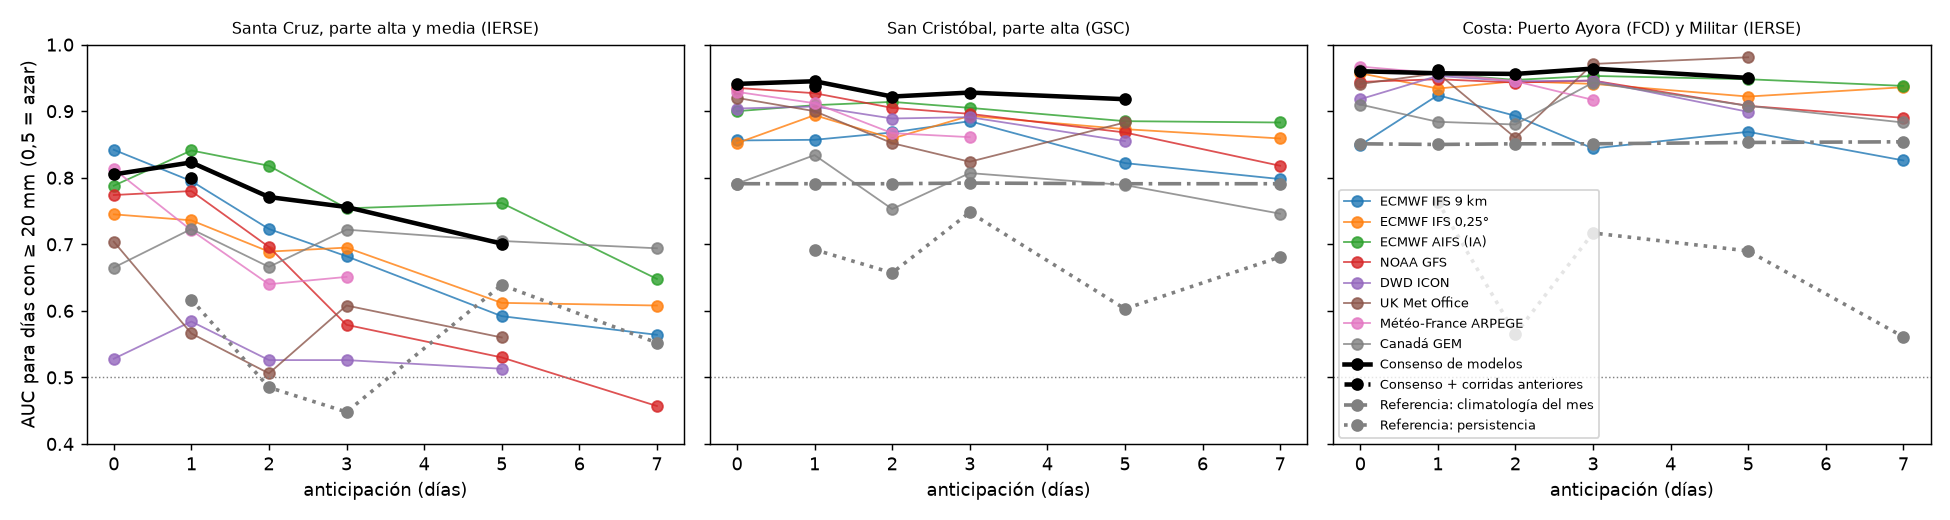
\includegraphics[width=\linewidth]{f_auc_20mm.png}
  \caption{AUC para los días con 20~mm o más según la anticipación, por modelo, para el consenso (negro) y para las referencias sin modelo (gris), en los tres grupos y en todo el año. 0,5 equivale al azar. Generada por \texttt{clima/scripts/07\_pronostico\_evaluacion.py}.}
  \label{fig:auc20}
\end{figure}

\begin{figure}[t]
  \centering
  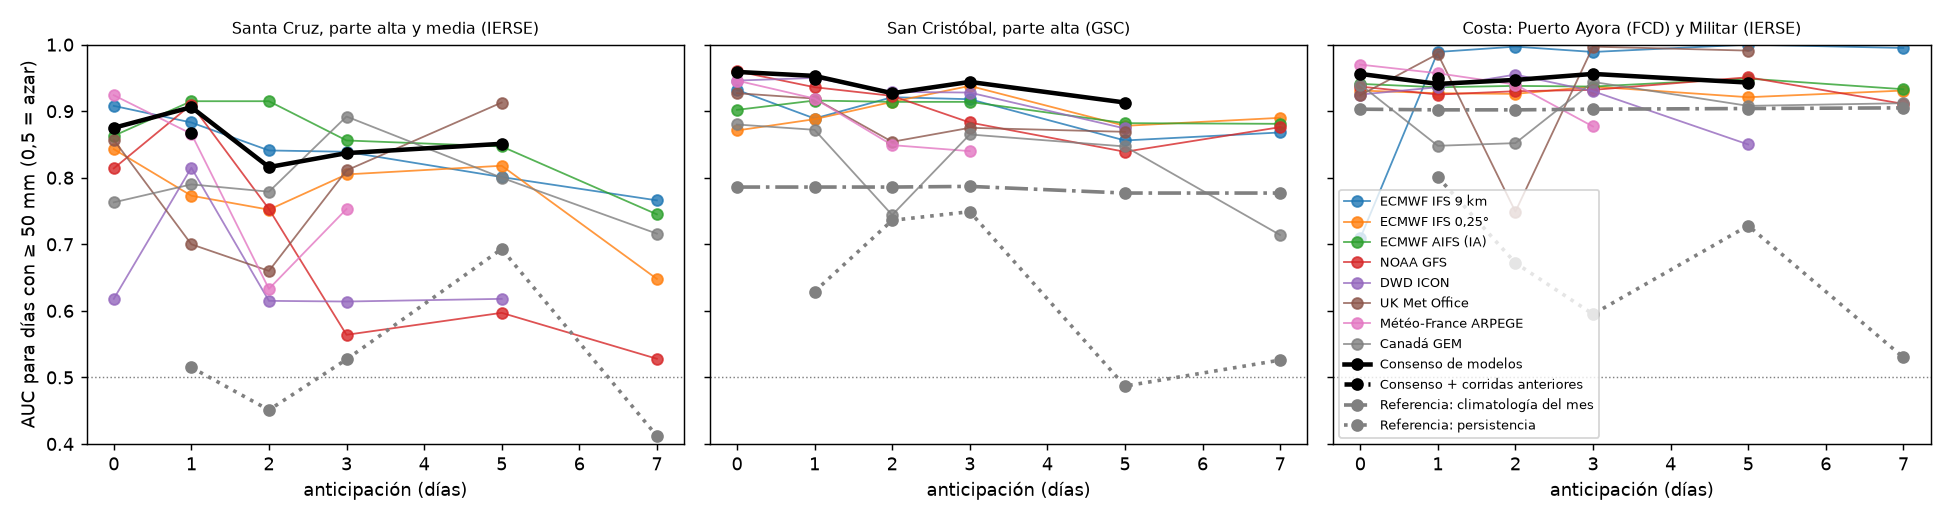
\includegraphics[width=\linewidth]{f_auc_50mm.png}
  \caption{Como la figura~\ref{fig:auc20}, para los días con 50~mm o más. Hay 25 estación-días con evento en San Cristóbal alta, 8 en la costa y 7 en Santa Cruz alta: las curvas son mucho más inciertas.}
  \label{fig:auc50}
\end{figure}

\subsection{Calibración}
La tabla~\ref{tab:cal} y la figura~\ref{fig:curvas} resumen las curvas logísticas de 20~mm. En validación cruzada, para hoy, la probabilidad mejora a la frecuencia climatológica en los tres grupos: BSS de 0,25 en la parte alta de San Cristóbal en temporada lluviosa, 0,14 en la parte alta de Santa Cruz en la garúa de 2026 y 0,10 en la costa en temporada lluviosa. A más anticipación la habilidad baja, sobre todo en Santa Cruz (0,06 para mañana).

En la costa, incluso con un consenso de 0,95, la probabilidad no pasa del 17\,\%: los días de lluvia fuerte son raros (4\,\% de los días en temporada lluviosa) y el consenso alto no basta para anticiparlos. Para 50~mm el BSS va de 0,00 en la costa a 0,16 en Santa Cruz (con solo 5 días), así que esa probabilidad solo se muestra en el detalle, marcada como \enquote{poco fiable}.

\begin{table}[ht]
  \centering\small
  \caption{Curvas logísticas para 20~mm o más: probabilidad según el consenso del grupo y habilidad en validación cruzada. Fuente: \texttt{clima/pronostico/fase0/calibracion\_logistica.csv}.}
  \label{tab:cal}
  \begin{tabularx}{\linewidth}{>{\raggedright\arraybackslash}Xcccccccc}
    \toprule
    Grupo y temporada & \makecell{Días $\geq 20$\\(de $n$)} & \makecell{Frec.\\normal} & Ant. & $a$ & $b$ & \makecell{$P$ con\\$\bar C = 0{,}80$} & \makecell{$P$ con\\$\bar C = 0{,}95$} & BSS \\
    \midrule
    San Cristóbal alta, lluviosa & 54 (388) & 14\,\% & 1 & $-7{,}93$ & 8,37 & 23\,\% & 51\,\% & 0,25 \\
    & & & 2 & $-7{,}04$ & 7,27 & 23\,\% & 47\,\% & 0,17 \\
    & & & 5 & $-7{,}04$ & 7,35 & 24\,\% & 49\,\% & 0,15 \\
    \addlinespace
    Costa, lluviosa & 17 (404) & 4\,\% & 1 & $-12{,}91$ & 11,94 & 3\,\% & 17\,\% & 0,10 \\
    & & & 2 & $-12{,}20$ & 11,16 & 4\,\% & 17\,\% & 0,10 \\
    & & & 5 & $-10{,}58$ & 8,98 & 3\,\% & 11\,\% & 0,08 \\
    \addlinespace
    Santa Cruz alta, garúa & 15 (148) & 10\,\% & 1 & $-5{,}79$ & 7,08 & 47\,\% & 72\,\% & 0,14 \\
    & & & 2 & $-4{,}98$ & 5,75 & 41\,\% & 62\,\% & 0,06 \\
    & & & 5 & $-4{,}90$ & 5,68 & 41\,\% & 62\,\% & 0,09 \\
    \bottomrule
  \end{tabularx}
  \par\vspace{3pt}\raggedright\footnotesize La frecuencia normal es la de la anticipación 1; a 5 días cambia algo porque la muestra es menor.
\end{table}

\begin{figure}[t]
  \centering
  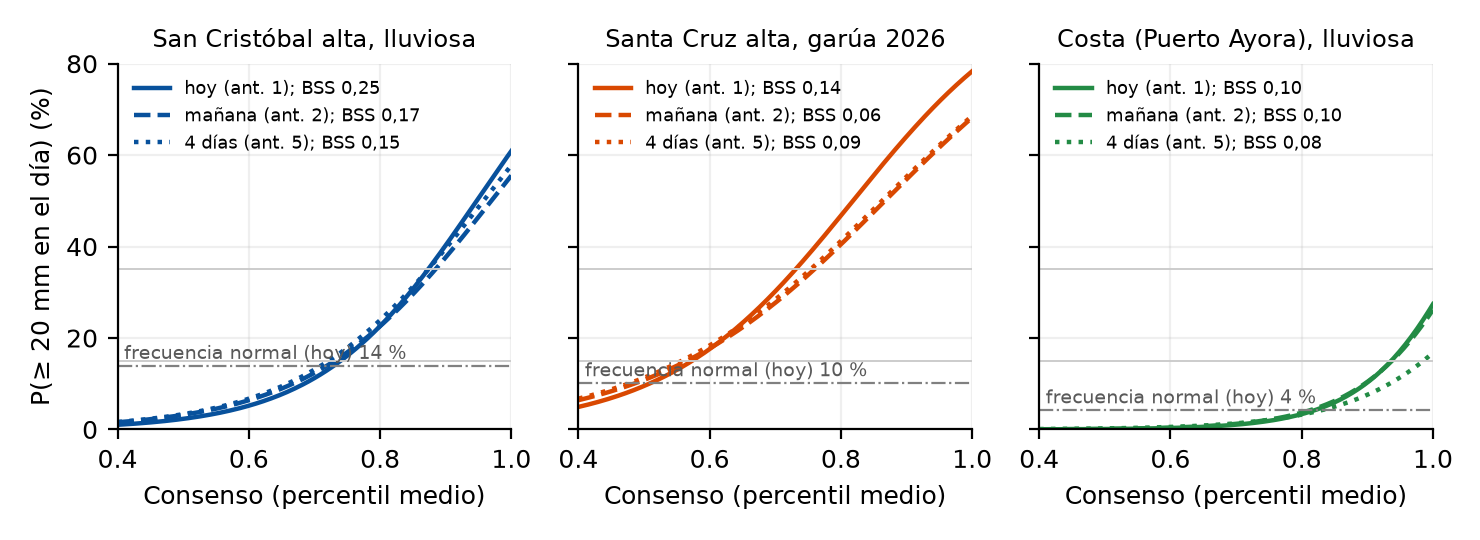
\includegraphics[width=\linewidth]{curvas_logisticas.png}
  \caption{Probabilidad de que alguna estación del grupo mida 20~mm o más según el consenso, para hoy, mañana y 4 días, con su BSS en validación cruzada. Líneas grises: cortes del 15 y el 35\,\% de los niveles; raya y punto: frecuencia normal. Figura de \texttt{informes/2026-08-pronostico/figuras.py} con los coeficientes de \texttt{calibracion\_logistica.csv}.}
  \label{fig:curvas}
\end{figure}

\subsection{Los niveles en validación cruzada}
La tabla~\ref{tab:niveles} y la figura~\ref{fig:fiabilidad} muestran qué pasó los días en que la señal, calculada sin esos días, estuvo en cada nivel. En la parte alta de San Cristóbal, con \enquote{señal alta} para hoy, hubo 20~mm o más en la mitad de los días; sin señal, solo en el 5\,\%. En la costa la señal nunca pasó de moderada: con ella hubo 20~mm o más en uno de cada seis días, y sin ella, en uno de cada 40.

\begin{table}[ht]
  \centering\small
  \caption{Frecuencia observada de 20 y 50~mm o más según el nivel publicado (validación cruzada). Fuente: \texttt{senal\_niveles.csv}.}
  \label{tab:niveles}
  \begin{tabular}{llccccc}
    \toprule
    Grupo y temporada & Día & Nivel & Días & \makecell{$P$ media\\anunciada} & \makecell{Con\\$\geq 20$~mm} & \makecell{Con\\$\geq 50$~mm} \\
    \midrule
    San Cristóbal alta, lluviosa & hoy & alta & 63 & 45\,\% & 49\,\% & 16\,\% \\
    & & moderada & 51 & 24\,\% & 20\,\% & 2\,\% \\
    & & sin señal & 274 & 4\,\% & 5\,\% & 2\,\% \\
    & mañana & alta & 46 & 43\,\% & 37\,\% & 15\,\% \\
    & & moderada & 83 & 24\,\% & 33\,\% & 5\,\% \\
    & & sin señal & 258 & 4\,\% & 4\,\% & 2\,\% \\
    \addlinespace
    Costa, lluviosa & hoy & moderada & 49 & 20\,\% & 16\,\% & 4\,\% \\
    & & sin señal & 355 & 2,5\,\% & 2,5\,\% & 2\,\% \\
    \addlinespace
    Santa Cruz alta, garúa 2026 & hoy & alta & 5 & 67\,\% & 3 de 5 & 2 de 5 \\
    & & moderada & 21 & 23\,\% & 19\,\% & 5\,\% \\
    & & sin señal & 122 & 5\,\% & 7\,\% & 2\,\% \\
    \bottomrule
  \end{tabular}
\end{table}

\begin{figure}[t]
  \centering
  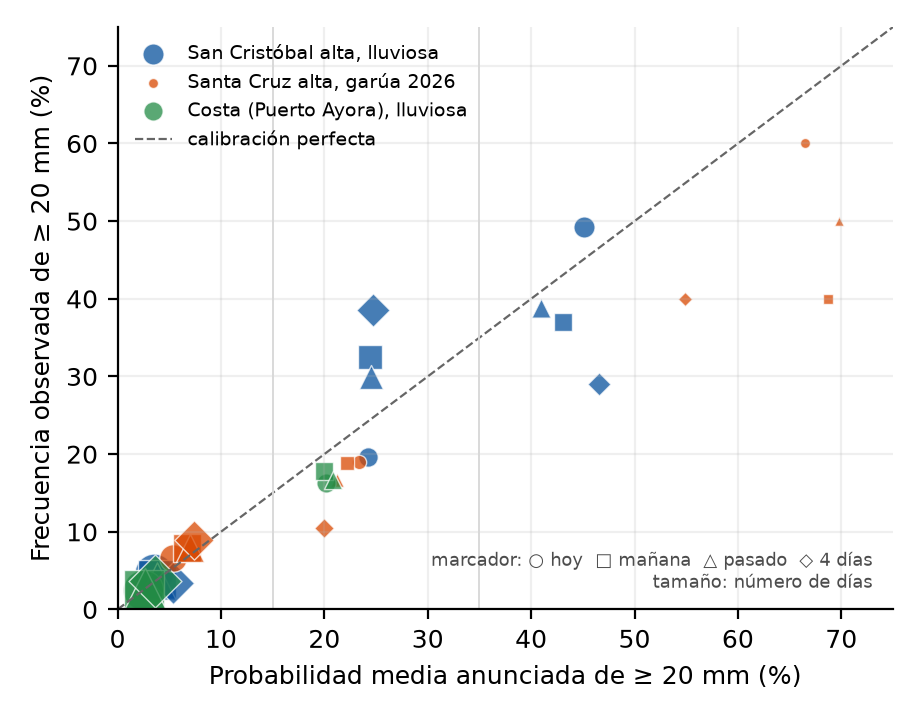
\includegraphics[width=0.62\linewidth]{fiabilidad.png}
  \caption{Diagrama de fiabilidad por niveles: probabilidad media anunciada frente a la frecuencia observada de 20~mm o más, en validación cruzada, para cada grupo, nivel y anticipación. Los puntos de Santa Cruz con probabilidad alta (4--5 días cada uno) quedan por debajo de la diagonal: sobreconfianza. Figura de \texttt{informes/2026-08-pronostico/figuras.py} con \texttt{senal\_niveles.csv}.}
  \label{fig:fiabilidad}
\end{figure}

\textbf{Sobreconfianza en Santa Cruz.} Con probabilidades altas la curva de Santa Cruz se pasa: los días con señal alta anuncian en promedio un 55--70\,\%, y llovió 20~mm o más solo en el 40--60\,\% de ellos (3 de 5 para hoy y 2 de 5 para mañana). Por eso la web redondea a múltiplos de 5\,\%, rotula la zona como \enquote{calibración provisional} y muestra al lado lo \enquote{normal en esta época}.

\subsection{Los días de lluvia fuerte}
La tabla~\ref{tab:fuertes} cuenta, para los días con 50~mm o más, en qué nivel estaba la señal. En la parte alta de San Cristóbal 10 de 15 tuvieron señal alta el mismo día y 7 desde la víspera. En la costa, 6 de 8 no tuvieron ninguna señal.

\begin{table}[ht]
  \centering\small
  \caption{Días con 50~mm o más en alguna estación del grupo, según el nivel de la señal (alta / moderada / sin señal). Validación cruzada. Fuente: \texttt{senal\_dias\_fuertes.csv}.}
  \label{tab:fuertes}
  \begin{tabular}{lcccc}
    \toprule
    Grupo & Días & Hoy & Mañana & 4 días \\
    \midrule
    San Cristóbal alta (lluviosa) & 15 & 10 / 1 / 4 & 7 / 4 / 4 & 4 / 6 / 2$^{*}$ \\
    Costa (lluviosa) & 8 & 0 / 2 / 6 & 0 / 2 / 6 & 0 / 0 / 3$^{*}$ \\
    Santa Cruz alta (garúa 2026) & 5 & 2 / 1 / 2 & 2 / 0 / 3 & 2 / 0 / 3 \\
    \bottomrule
  \end{tabular}
  \par\vspace{3pt}\raggedright\footnotesize $^{*}$ A 5 días de anticipación hay menos días con archivo de todos los modelos.
\end{table}

La tabla~\ref{tab:eventos} sigue los cinco días de lluvia fuerte de Santa Cruz en 2026. Al calibrar se dejó fuera todo octubre, así que la señal de octubre es la que se habría publicado sin conocer esos días. El 23 y el 30-oct tuvieron \enquote{señal alta} desde cuatro días antes. El 3-oct (68~mm) y el 4-oct (44~mm) no tuvieron señal, y el 14-jun (65~mm) solo tuvo señal moderada el mismo día.

\begin{table}[ht]
  \centering\small
  \caption{Probabilidad de 20~mm o más, en validación cruzada, para los días de lluvia fuerte de la parte alta de Santa Cruz en 2026. \enquote{Medido}: máximo de las estaciones del grupo (red IERSE-WSN).}
  \label{tab:eventos}
  \begin{tabular}{lccccc}
    \toprule
    Día & Medido & Hoy & Mañana & Pasado & 4 días \\
    \midrule
    30-oct & 238~mm & 82\,\% & 79\,\% & 77\,\% & 65\,\% \\
    23-oct & 97~mm & 61\,\% & 55\,\% & 58\,\% & 52\,\% \\
    14-jun & 65~mm & 32\,\% & 13\,\% & 16\,\% & 12\,\% \\
    3-oct & 68~mm & 10\,\% & 5\,\% & 8\,\% & 13\,\% \\
    4-oct & 44~mm & 4\,\% & 3\,\% & 7\,\% & 14\,\% \\
    \bottomrule
  \end{tabular}
\end{table}

\textbf{Prueba de punta a punta.} Se reconstruyeron varios días de 2026 con el código de producción (\texttt{pronostico.py}) a partir del archivo en los puntos de cada zona. En la cuenca alta de La Cascada, el 30-oct sale \enquote{señal alta} del día 0 al 4 (55--69\,\%) y el 23-oct también (38--54\,\%). El 3-oct sale \enquote{sin señal} hasta el día 2 y \enquote{moderada} a 4 días (17\,\%). El 15-sep, un día seco, sale \enquote{sin señal} (2--4\,\%). Esa prueba descubrió un fallo de la primera versión: con un \enquote{sin señal} fijo en la garúa de la costa, Puerto Ayora daba 0\,\% el 30-oct con el consenso en 0,97, cuando el INAMHI midió 94~mm ese día y 135~mm el 31 (días continentales). Con la curva prestada de la temporada lluviosa, ese día sale \enquote{señal moderada} (${\approx}\,20$\,\%). En 2024--2026, esa curva no habría dado ninguna señal alta en garúa, y solo señal moderada en dos días sin lluvia fuerte; tampoco habría anticipado los dos días de 20~mm o más de la garúa de San Cristóbal (3--6\,\%).

\subsection{Intensidad en 3 horas}
Con los datos de 5~min de la red IERSE-WSN (abril--octubre de 2026) hay 8 días con un máximo de 20~mm o más en 3~h. Los modelos los distinguen algo (AUC de 0,6--0,9 según el modelo y la anticipación; \texttt{metricas\_3h.csv}), pero en milímetros ninguno se acerca con un día de anticipación: el máximo es de 23~mm (IFS de 9~km), frente a 118~mm medidos en 3~h el 30-oct. La corrida más reciente del IFS de 9~km sí dio un pico de 98~mm en 3~h, pero entre las 03:00 y las 06:00 del 31-oct, unas 8~h después del pico medido y durante un corte de transmisión de la red, así que no se puede verificar. No se publica, por tanto, ningún nivel de inundación pronosticado: la regla de inundación (informe 2026-07) sigue usando solo lluvia medida.

\subsection{Lo que se publica}
Con estos resultados la plataforma publica, para hoy y los cuatro días siguientes, la probabilidad de 20~mm o más por zona, en tres niveles con colores neutros (no de alerta), junto a lo \enquote{normal en esta época} y rotulada como experimental y no oficial. No se publican los milímetros de los modelos como cantidad esperada, ni la probabilidad de 50~mm en los recuadros. El servicio en vivo (\texttt{clima/recolector/pronostico.py}) revisa cada hora si hay corridas nuevas, deja fuera las de más de 30~h y exige al menos 5 modelos. Los conjuntos (IFS ENS, AIFS ENS, GEFS, ICON-EPS y MOGREPS-G) se archivan para calibrarlos más adelante y por ahora solo muestran en qué bloques de 6~h de las próximas 72~h se concentra la lluvia.

% =====================================================================
\section{Discusión y limitaciones}

\textbf{Discriminar no es pronosticar cantidades.} Los modelos globales aportan información real sobre \emph{qué días} son propensos a lluvia fuerte, pero no sobre cuánto ni a qué hora. Esa información solo se vuelve utilizable al calibrarla con lluvia medida, y su habilidad, medida por el BSS (0,06--0,25), es modesta: la mayor parte de la incertidumbre del día sigue ahí. Un \enquote{sin señal} no garantiza un día sin lluvia fuerte, como muestran el 3 y el 4-oct.

\textbf{Santa Cruz tiene una muestra pequeña.} Su calibración se apoya en siete meses de la red IERSE-WSN (25-abr a 31-oct de 2026), con 15 días-grupo de 20~mm o más y 5 de 50~mm o más, casi todos en un octubre anómalo por El Niño. En temporada lluviosa toma prestada la curva de San Cristóbal, sin evidencia local de que valga. Además, dos de sus tres estaciones tienen dudas de funcionamiento (\issue{56}), sus cortes de transmisión hacen que los totales sean mínimos y el balancín subestima por encima de 50~mm/h.

\textbf{La costa tiene poca habilidad.} La probabilidad nunca pasó del 30\,\%, y 6 de 8 días con 50~mm o más no tuvieron señal. Los chubascos que dan lluvia fuerte en la costa parecen ser más locales que lo que una celda de 25~km representa.

\textbf{Sobreconfianza a probabilidades altas} en Santa Cruz (figura~\ref{fig:fiabilidad}): con 4--5 días por punto, la curva no está bien determinada en su extremo. Es un riesgo de comunicación: un 70\,\% puede leerse como casi seguro cuando la frecuencia observada fue del 40--60\,\%.

\textbf{Diferencias entre la evaluación y el servicio en vivo.} En la evaluación el consenso tuvo de 5 a 7 modelos; en vivo siempre tendrá 7. La climatología de cada modelo se calculó con todo el archivo, incluido el periodo evaluado; la revisión recalculó el consenso con percentiles que excluyen el bloque evaluado y el BSS no cambió (0,200 frente a 0,202). Que \enquote{hoy} y \enquote{mañana} en vivo se comporten como las anticipaciones 1 y 2 del archivo está por comprobar con los pronósticos archivados en vivo.

\textbf{Otras limitaciones.} La garúa de la costa y de San Cristóbal no está calibrada (0 y 2 eventos). Isabela no tiene estaciones. La serie del GSC tiene años con huecos y no es pública, por lo que la serie con validación cruzada no se versiona. La FCD es un pluviómetro manual de lectura diaria. Los conjuntos no se pudieron evaluar, porque Open-Meteo no guarda sus corridas viejas por anticipación.

% =====================================================================
\section{Conclusiones y trabajo futuro}
\begin{enumerate}
  \item En milímetros, los modelos globales no sirven para la lluvia fuerte en Galápagos: en los días extremos se quedan decenas de veces por debajo de lo medido.
  \item El consenso de percentiles sí distingue los días con 20~mm o más: AUC de 0,85--0,92 hasta tres días en temporada lluviosa, frente a 0,64 de la climatología.
  \item Calibrado con una regresión logística, mejora a la frecuencia climatológica en todos los grupos para hoy (BSS de 0,10 a 0,25 en validación cruzada).
  \item La señal anticipó desde cuatro días antes el 23 y el 30-oct en Santa Cruz, pero no el 3 y el 4-oct; en la costa falló en 6 de 8 días con 50~mm o más.
  \item No pronostica la intensidad en 1--3~h; esa escala corresponde a las estaciones y a la vigilancia satelital.
\end{enumerate}

Quedan pendientes:
\begin{itemize}
  \item recalibrar con los pronósticos archivados en vivo y comprobar la correspondencia entre anticipación y día de la web;
  \item recalibrar Santa Cruz con su primera temporada lluviosa medida (enero--mayo de 2027);
  \item calibrar los conjuntos (IFS ENS, AIFS ENS) cuando haya al menos una temporada archivada;
  \item combinar la señal diaria con la vigilancia satelital GOES-19 de 0--6~h (trabajo aparte, futuro informe 2026-09) y con la lluvia satelital GPM IMERG (\issue{20});
  \item la licencia de los datos del GSC (\issue{46}) y la revisión en campo de las estaciones de Santa Cruz (\issue{56}).
\end{itemize}

\section*{Disponibilidad de datos y código}
{\small Todo el procesamiento es reproducible desde el repositorio público \emph{mayait/sosgalapagos-datos}. Los endpoints de Open-Meteo no se publican: viven en \texttt{clima/privado/fuentes.env}, fuera del control de versiones.
\begin{itemize}
  \item \texttt{clima/scripts/06\_pronostico\_archivo.py}: descarga del archivo de pronósticos (no versionado, ${\approx}\,30$~MB);
  \item \texttt{clima/scripts/07\_pronostico\_evaluacion.py}: evaluación, calibración y figuras; escribe \texttt{clima/pronostico/fase0/} (\texttt{metricas.csv}, \texttt{metricas\_3h.csv}, \texttt{calibracion\_logistica.csv}, \texttt{senal\_niveles.csv}, \texttt{senal\_dias\_fuertes.csv}, \texttt{resumen.json}) y \texttt{clima/recolector/pronostico\_calibracion.json};
  \item \texttt{clima/recolector/pronostico.py} y \texttt{pronostico\_reglas.json}: servicio en vivo, niveles y textos;
  \item \texttt{clima/pronostico/LEEME.md} y \texttt{fase0/informe.md}: documentación y evaluación detallada;
  \item \texttt{informes/2026-08-pronostico/figuras.py}: figuras propias de este informe.
\end{itemize}
Los pares diarios con la serie del GSC y la serie con validación cruzada no se versionan, porque contienen datos del GSC sin licencia publicada. Este informe se compila con \texttt{informes/compilar.sh 2026-08-pronostico}.\par}

\bibliographystyle{sosg}
\bibliography{referencias,bib-2026-08}

\end{document}
